\documentclass{article}
% generated by Madoko, version 1.0.0-rc5
%mdk-data-line={1}


\usepackage[heading-base={2},section-num={False},bib-label={True}]{madoko2}


\begin{document}



{\mdfontfamily{SimSun}
%mdk-data-line={11}
\mdxtitleblockstart{}
%mdk-data-line={11}
\mdxtitle{\mdline{11}统计学习笔记}%mdk
\mdxauthorstart{}
%mdk-data-line={16}
\mdxauthorname{\mdline{16}Stanley Wu}%mdk

%mdk-data-line={19}
\mdxauthoraddress{\mdline{19}GmaxInfo}%mdk

%mdk-data-line={22}
\mdxauthoremail{\mdline{22}bleedtodry@hotmail.com}%mdk
\mdxauthorend\mdtitleauthorrunning{}{}\mdxtitleblockend%mdk
\mdline{13}
\begin{mdtoc}%mdk

\section*{Contents}\label{sec-contents}%mdk%mdk

\begin{mdtocblock}%mdk

\mdtocitemx{section}{\mdref{section}{1.\hspace*{0.5em}线性模型}}%mdk

\begin{mdtocblock}%mdk

\mdtocitemx{section}{\mdref{section}{1.1.\hspace*{0.5em}特征选择}}%mdk
%mdk
\end{mdtocblock}%mdk

\mdtocitemx{section}{\mdref{section}{2.\hspace*{0.5em}分类算法}}%mdk

\begin{mdtocblock}%mdk

\mdtocitemx{sec-logistic-regression}{\mdref{sec-logistic-regression}{2.1.\hspace*{0.5em}Logistic Regression}}%mdk

\mdtocitemx{sec-linear-discriminant-analysis}{\mdref{sec-linear-discriminant-analysis}{2.2.\hspace*{0.5em}Linear Discriminant Analysis}}%mdk
%mdk
\end{mdtocblock}%mdk

\mdtocitemx{section}{\mdref{section}{3.\hspace*{0.5em}重抽样}}%mdk

\begin{mdtocblock}%mdk

\mdtocitemx{sec-cross-validation}{\mdref{sec-cross-validation}{3.1.\hspace*{0.5em}Cross-Validation}}%mdk

\begin{mdtocblock}%mdk

\mdtocitemx{sec-leave-one-out-cross-validation}{\mdref{sec-leave-one-out-cross-validation}{3.1.1.\hspace*{0.5em}Leave-One-Out Cross-Validation}}%mdk

\mdtocitemx{sec-k-folder-cross-validation}{\mdref{sec-k-folder-cross-validation}{3.1.2.\hspace*{0.5em}k-Folder Cross-Validation}}%mdk
%mdk
\end{mdtocblock}%mdk

\mdtocitemx{sec-bootstrap}{\mdref{sec-bootstrap}{3.2.\hspace*{0.5em}Bootstrap}}%mdk
%mdk
\end{mdtocblock}%mdk
%mdk
\end{mdtocblock}%mdk
%mdk
\end{mdtoc}%mdk

%mdk-data-line={15}
\section{\mdline{15}1.\hspace*{0.5em}\mdline{15}线性模型}\label{section}%mdk%mdk

%mdk-data-line={16}
\subsection{\mdline{16}1.1.\hspace*{0.5em}\mdline{16}特征选择}\label{section}%mdk%mdk

%mdk-data-line={18}
\section{\mdline{18}2.\hspace*{0.5em}\mdline{18}分类算法}\label{section}%mdk%mdk

%mdk-data-line={19}
\subsection{\mdline{19}2.1.\hspace*{0.5em}\mdline{19}Logistic Regression}\label{sec-logistic-regression}%mdk%mdk

%mdk-data-line={20}
\noindent\mdline{20}基本模型:%mdk
\label{}%mdk
\noindent\mdline{21}\mdmathtag{(1)}\mdline{21}
\noindent\[%mdk-data-line={22}
p(X)=\frac{e^{\beta_0+\beta_{1X}}}{1+e^{\beta_0+\beta_{1X}}}
\]%mdk
\noindent\mdline{24}Log-odds logit:
\label{}%mdk
\noindent\mdline{25}\mdmathtag{(2)}\mdline{25}
\noindent\[%mdk-data-line={26}
\log(\frac{p(X)}{1-p(X)}) = \beta_0+\beta_{1X}
\]%mdk
\noindent\mdline{28}最大似然参数估计:
\label{}%mdk
\noindent\mdline{29}\mdmathtag{(3)}\mdline{29}
\noindent\[%mdk-data-line={30}
  \zeta(\beta_0,\beta_1)= \prod_{i:y_i=1}p(x_i)\prod_{i:y_i=0}(1-p(x_i))
\]%mdk

%mdk-data-line={32}
\subsection{\mdline{32}2.2.\hspace*{0.5em}\mdline{32}Linear Discriminant Analysis}\label{sec-linear-discriminant-analysis}%mdk%mdk

%mdk-data-line={33}
\noindent\mdline{33}Logistic Regression适用于二元离散回归,当因变量大于2个时,使用LDA%mdk

%mdk-data-line={34}
\section{\mdline{34}3.\hspace*{0.5em}\mdline{34}重抽样}\label{section}%mdk%mdk

%mdk-data-line={35}
\subsection{\mdline{35}3.1.\hspace*{0.5em}\mdline{35}Cross-Validation}\label{sec-cross-validation}%mdk%mdk

%mdk-data-line={36}
\subsubsection{\mdline{36}3.1.1.\hspace*{0.5em}\mdline{36}Leave-One-Out Cross-Validation}\label{sec-leave-one-out-cross-validation}%mdk%mdk

%mdk-data-line={37}
\noindent\mdline{37}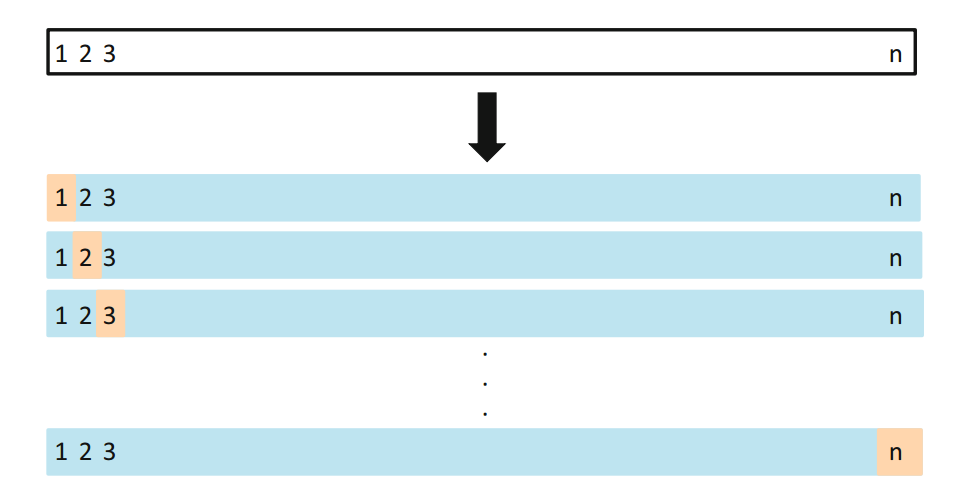
\includegraphics[keepaspectratio=true,width=\dimmin{}{\dimwidth{0.80}}]{images/LOOCV}{}\mdline{37}%mdk
\label{}%mdk
\noindent\mdline{40}\mdmathtag{(4)}\mdline{40}
\noindent\[%mdk-data-line={41}
  CV=\frac{1}{n}\sum_{i=1}^{n}MSE_i
\]%mdk

%mdk-data-line={43}
\subsubsection{\mdline{43}3.1.2.\hspace*{0.5em}\mdline{43}k-Folder Cross-Validation}\label{sec-k-folder-cross-validation}%mdk%mdk
\label{}%mdk
\noindent\mdline{44}\mdmathtag{(5)}\mdline{44}
\noindent\[%mdk-data-line={45}
CV_{(K)}=\sum_{k=1}^{K}\frac{n_k}{n}MSE_k
\]%mdk
\noindent\mdline{47}LOOCV是k-Folder CV的一种特殊情况,即\mdline{47}$k=n$\mdline{47}。

%mdk-data-line={48}
\subsection{\mdline{48}3.2.\hspace*{0.5em}\mdline{48}Bootstrap}\label{sec-bootstrap}%mdk%mdk

%mdk-data-line={49}
\noindent\mdline{49}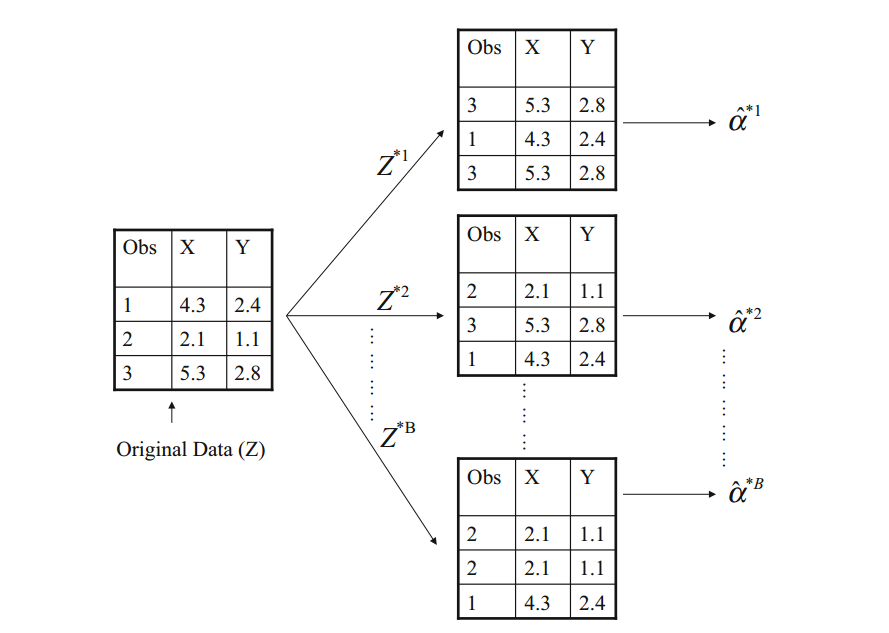
\includegraphics[keepaspectratio=true,width=\dimmin{}{\dimwidth{0.70}}]{images/Bootstrap}{}\mdline{49}%mdk

%mdk-data-line={54}
\begin{mdbmargintb}{4em}{}%mdk
\begin{mdflushright}%mdk
{\tiny\mdline{55}Created with~\href{https://www.madoko.net}{Madoko.net}.}%mdk
\end{mdflushright}%mdk
\end{mdbmargintb}%mdk
}%mdk


\end{document}
